\subsection{Les Modèles de Données dans les Musées : Un État des Lieux}
\textbf{Contexte Actuel des Modèles de Données dans les Musées}\newline

Dans le domaine muséal, la question de la normalisation et de la structuration des données est devenue cruciale à mesure que les institutions cherchent à améliorer la gestion et la diffusion de leurs collections. Plusieurs modèles de données ont été développés pour répondre à ces besoins, chacun avec ses spécificités et ses objectifs. Parmi les plus notables utilisés en France, on trouve le Dublin Core, l'export Joconde, le CIDOC CRM et diverses ontologies spécifiques.\newline

Le Dublin Core est un schéma de métadonnées simple, il peut être utilisé dans le milieu muséal pour décrire les objets culturels. Il est particulièrement apprécié pour sa simplicité et sa flexibilité, ce qui permet une adoption facile par les institutions, même celles qui disposent de ressources limitées.\newline


\begin{longtable}{|p{4cm}|p{4cm}|p{8cm}|}
\hline
\textbf{Élément} & \textbf{Élément (anglais)} & \textbf{Commentaire} \\
\hline
1. Titre (métadonnée) & Title & Nom donné à la ressource \\
\hline
2. Créateur (métadonnée) & Creator & Nom de la personne, de l'organisation ou du service responsable de la création du contenu de la ressource \\
\hline
3. Sujet (métadonnée) ou mots clés & Subject & Thème du contenu de la ressource (mots clés, expressions, codes de classification) \\
\hline
4. Description (métadonnée) & Description & Présentation du contenu de la ressource (résumé, table des matières, représentation graphique du contenu, texte libre) \\
\hline
5. Éditeur & Publisher & Nom de la personne, de l'organisation ou du service responsable de la mise à disposition ou de la diffusion de la ressource \\
\hline
6. Contributeur & Contributor & Nom de la personne, de l'organisation ou du service responsable de contributions au contenu de la ressource \\
\hline
7. Date (métadonnée) & Date & Date de création ou de mise à disposition de la ressource \\
\hline
8. Type & Type & Nature ou genre de la ressource (catégories, fonctions, genres généraux, niveaux d'agrégation du contenu) \\
\hline
9. Format & Format & Manifestation physique ou numérique de la ressource \\
\hline
10. Identifiant de la ressource & Identifier & Référence univoque à la ressource dans un contexte donné (URI, ISBN) \\
\hline
11. Source & Source & Référence à une ressource dont la ressource décrite est dérivée (URI) \\
\hline
12. Langue (métadonnée) & Language & Langue du contenu intellectuel de la ressource \\
\hline
13. Relation (métadonnée) & Relation & Référence à une ressource apparentée \\
\hline
14. Couverture (métadonnée) & Coverage & Couverture spatio-temporelle de la ressource (domaine d'application) \\
\hline
15. Gestion de droits (métadonnée) & Rights & Informations sur les droits associés à la ressource (IPR, copyright, etc.) \\
\hline
\end{longtable}


L'export Joconde, quant à lui, est un format spécifiquement développé pour les musées français. Il permet de structurer les informations relatives aux objets des collections de manière à ce qu'elles puissent être intégrées dans la base Joconde, le catalogue collectif des musées de France. Ce format est essentiel pour la mutualisation des données à l'échelle nationale, assurant ainsi une visibilité accrue des collections et une diffusion accrue et efficace.\newline

Le CIDOC CRM (Conceptual Reference Model) que nous avons déjà présenté est un modèle conceptuel élaboré par le Comité international pour la documentation (CIDOC) du Conseil international des musées (ICOM). Il vise à modéliser les relations complexes entre les objets, les événements et les personnes dans le domaine du patrimoine culturel.\newline

Enfin, les ontologies spécifiques aux musées, comme celles développées pour les objets ethnographiques ou les œuvres d'art, permettent de structurer les données en fonction des particularités de chaque type de collection. Ces ontologies facilitent l'intégration des données dans des systèmes de gestion complexes, tout en assurant une cohérence et une précision accrues.\newline

\textbf{Exemples Pratiques et Impact sur la Qualité des Données}\newline

Au cours de notre stage nous avons rencontré différents cas d’usages. En effet, dans le cadre de notre mission au sein du DPNC (sous direction du Service du numérique, Département du numérique pour la transformation des politiques culturelles et de l'administration des données)nous avons participé à l’animation du réseau des agrégateurs intermédiaires. Ces entités agrègent les données de plusieurs institutions culturelles et les diffusent sur des portails et des sites internets. Ces agrégateurs réunissent les données d'institutions selon des critères qui peuvent être thématiques ou géographiques. \newline

Nous avons notamment pu échanger avec des représentants du portail Bretania, qui agrège et diffuse des données d'institutions culturelles en Bretagne telles que  la Cinémathèque de Bretagne, les différents musées et les archives municipales, entre autres. La Base Aliénor et la DRAC PACA, réunissent eux aussi des données relevant du patrimoine culturel à l’échelle de leur région. Nous avons également échangé avec des représentants du projet de portail thématique Graph Ethno, un portail des collections des écomusées et musées de société en France qui à pour objectif de créer un réseau de valorisation numérique des collections de ces institutions. \newline

Dans le projet d’agrégation du ministère, le but n’est pas de se limiter aux institutions muséales, c’est pour cette raison que nous avons également pu échanger avec des représentants de la Réunion des Opéras de France et de la Philharmonie de Paris. 
Chacun des agrégateurs que nous avons pu rencontrer à des pratiques différentes pour agréger et gérer ses données. Voici quelques exemples auxquels nous avons fait face. \newline

Le cas de la Réunion des Opéras de France (ROF) et CapData Opéra : 
La ROF mène depuis 2O22 le projet CapData Opéra, c’est un projet qui utilise les technologies du Web sémantique comme fondement d’une solution de structuration et de diffusion des données culturelles capable de répondre aux besoins des institutions. Cette initiative est portée par la ROF avec le soutien du Ministère de la Culture et de plusieurs partenaires techniques, tels que Logilab (une société qui développe des logiciels, de préférence libres, et propose du conseil et des formations dans les domaines du web sémantique et de l'informatique scientifique). Cette solution de mutualisation permet d’interroger les données produites par plusieurs acteurs du domaine pour, par exemple, connaître la programmation et la circulation d’une œuvre ou d’une production entre plusieurs maisons d’opéra. Ce projet réunit les donnés de six maisons d’opéra et s’appuie sur les technologies du Web sémantique et notamment sur le standard RDF (Resource Description Framework). Ce projet a aboutit à la publication de l‘ontologie CapData Opéra. \newline
L'objectif est de centraliser et de standardiser les informations, facilitant ainsi leur partage et leur utilisation par des publics variés, incluant les opéras, les développeurs, et les acteurs culturels.\newline

Les maisons d'opéra gèrent quotidiennement des données multiples, notamment sur leur programmation, les artistes, et les productions. Cependant, ces données sont souvent stockées dans des systèmes distincts et non interopérables, rendant difficile leur croisement et leur réutilisation à grande échelle. L'absence de standards communs pour identifier les œuvres, les artistes, ou les productions de spectacles vivants constitue un frein majeur à leur diffusion. À titre d'exemple, il n'existe pas d'équivalent à l'ISBN (livres) ou à l'ISRC (industrie musicale) pour identifier les productions de spectacle vivant, compliquant la tâche des maisons d’opéra souhaitant partager leurs données avec d’autres plateformes. \newline

Le projet CapData Opéra se donne pour mission de résoudre ces problèmes d'interopérabilité en créant une infrastructure mutualisée qui permet aux maisons d’opéra de publier et de partager leurs données de manière standardisée. Cette infrastructure repose sur les technologies du Web Sémantique et notamment sur le standard RDF (Resource Description Framework), un format conçu pour représenter les données de manière structurée et facilitant leur interconnexion.
Le projet vise à répondre à plusieurs enjeux clés :
Interopérabilité accrue des données : permettre aux maisons d'opéra de partager facilement leurs informations avec d'autres institutions et acteurs culturels.
Réduction des saisies manuelles : minimiser les doublons et les erreurs de saisie en automatisant la structuration et la diffusion des données.
Facilitation de la découvrabilité : accroître la visibilité des œuvres, artistes, et productions auprès des publics via des plateformes numériques, des moteurs de recherche, ou des services innovants.
Souveraineté des données : permettre à chaque maison d'opéra de conserver le contrôle sur ses propres données tout en facilitant leur partage avec d'autres. \newline

Pour structurer et diffuser les données, CapData Opéra s'appuie sur une ontologie dédiée qui définit un vocabulaire commun entre les différents opéras. Cette ontologie est conçue pour s'aligner avec des modèles de données existants, notamment schema.org, utilisé pour la découvrabilité sur le web, et l’ontologie IFLA-LRM, bien adaptée aux ressources bibliographiques. Cependant, certaines lacunes ont été identifiées dans ces modèles, notamment en ce qui concerne la description fine des productions artistiques, ce qui a conduit au développement d’une ontologie propre à CapData Opéra.
Une partie clé du projet repose sur le développement d’un outil appelé Rodolf, conçu pour suivre la publication et la structuration des données RDF. Rodolf permet aux maisons d'opéra de suivre les fichiers de données publiés, d'identifier d'éventuelles erreurs, et de vérifier la validité des données à travers un ensemble de règles SHACL (Shapes Constraint Language). En outre, un kit de développement logiciel (SDK) a été mis à disposition pour faciliter l’export des données en RDF, même pour les développeurs peu familiers avec les technologies du Web Sémantique. \newline

Depuis son lancement en 2022, CapData Opéra a d'abord été testé avec l'Opéra National de Bordeaux et d'autres partenaires. Les premiers résultats montrent une nette amélioration de la capacité à croiser les données entre les opéras et à diffuser les informations de manière cohérente et automatisée. Le projet a également permis de créer des liens avec des initiatives internationales similaires, notamment dans le domaine des arts vivants et du spectacle.
En plus de faciliter la publication et la circulation des données, cette approche a aussi permis d'améliorer la qualité des informations stockées par chaque maison d'opéra. Grâce aux outils développés, les opéras peuvent désormais enrichir leurs propres bases de données avec des informations normalisées, telles que les identifiants ISNI (International Standard Name Identifier) pour les artistes. \newline

Le projet CapData Opéra représente une avancée significative pour la gestion des données dans le secteur des arts vivants, et notamment pour les maisons d'opéra. En s’appuyant sur les technologies du Web Sémantique et une ontologie dédiée, il facilite la standardisation et la diffusion des données tout en respectant la souveraineté de chaque institution. À terme, cette initiative pourrait s’étendre à d’autres types d’institutions culturelles, comme les théâtres, et contribuer à une meilleure visibilité des créations artistiques à travers les plateformes numériques et les nouveaux modes de diffusion.

Le projet est encore en phase d’expérimentation et de développement, mais les résultats obtenus jusqu'à présent sont prometteurs, avec des perspectives de déploiement à grande echelle. \footcite{CapData_Opera}

\begin{figure}[h!]
	\centerline{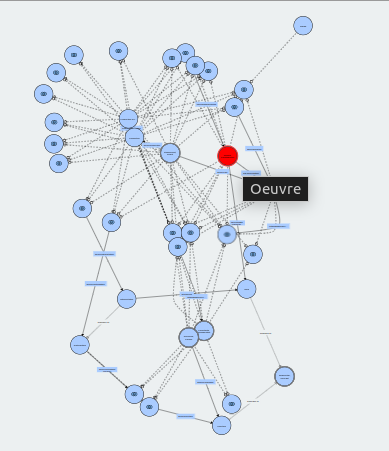
\includegraphics[width=\textwidth]{medias/capData_opera.png}}
	\caption{Apperçu du graphe de données de l'ontologie Capdata Opéra}
\end{figure}

La création d'ontologies spécifiques est également envisagée dans d'autres domaines tels que les collections d'ethnographie avec le projet GraphEthno, bien que ce dernier soit toujours en cours de développement.  Ce processus serait une solution cohérente avec la complexité des données générées par certaines de leurs institutions partenaires. Lors de nos premiers échanges c’est le Dublin Core qui leurs semblait le plus approprié pour porter les données collectées, c’est donc sous ce format que nous avons étudié leur cas. Le projet étant toujours en cours nous avons pu voir au cours des mois une évolution dans les réflexions et un intérêt pour le LIDO apparaître. \newline

Il est tout de même important de rappeler que tous les agrégateurs intermédiaires n’ont pas pour objectif de créer des ontologies. Bon nombre d’entre eux se basent sur des formats de données plus simples et choisis en fonction des données dont ils disposent. La Base Aliénor, par exemple, récupère les données en suivant les champs proposés par le format de l’export Joconde en y ajoutant des champs proposés par le Darwin Core. Le Darwin Core est une extension du Dublin Core, utilisée pour décrire avec plus de précision des objets de biodiversité.\newline

La plupart des agrégateurs intermédiaires que nous avons rencontrés n’utilisent pas de format de données standard. En effet pour produire leurs données ils s’appuient sur les informations dont ils disposent déjà dans leurs inventaires, catalogues et registres, ainsi que sur les possibilités proposées par l’éditeur de leur base de données. Le format de leurs données est donc souvent dicté par l’outil utilisé par l’institution. \newline

En conclusion, l'utilisation de modèles de données dans les musées est essentielle pour assurer la qualité, la cohérence et la diffusion des informations sur les collections. Chaque modèle a ses avantages et ses limites, mais leur adoption permet de répondre aux besoins spécifiques des musées tout en assurant une interopérabilité accrue à l'échelle nationale et internationale. Malgrés cette affirmation, nous sommes forcé de constater que, même si quleques projets montrent une évolution dans les pratiques, la majorité des données collectées par les agrégateurs intermédiaires ne suivent pas de standards communs. Les données muséales prennent surtout la forme qui est facilitée par l'outil de gestion de chaque institution utilise. 

